%%% EC-mix.tex
% \documentclass[UTF8]{ctexart}
% \begin{document}
%     你好,world!
% \end{document}

%%% xeCJK-demo.tex
%%% 没报错,没警告。
% \documentclass{article}
% \usepackage{xeCJK}
% \setCJKmainfont{SimSun}
% \begin{document}
%     你好世界。I love you.
%     你好我爱ni
% \end{document}

%%% Microsoft fonts, use fontspec
% \documentclass{article}
% \usepackage{fontspec}
% \usepackage{xeCJK}
% \setCJKmainfont{Microsoft JhengHei UI}
% \setCJKfamilyfont{YaHei}{Microsoft YaHei UI}
% \begin{document}
%     This is a document mostly in English, but containing a few words in Chinese characters.
%     大豊饒諸衆善法
%     瞋怒
% \CJKfamily{YaHei}
%     大豊饒諸衆善法
%     瞋怒
% \end{document}

%%% Sectioin_Paragraph.tex
% \documentclass{article}
% \usepackage{xeCJK}
% \setCJKmainfont{SimSun}
% \title{你好,标题}
% \author{Delayless}
% \date{\today}
% \begin{document}
% \maketitle
% \section{你好章节}
% 章节是书本内的最大单位
% \subsection{你好,子章节}
% 子章节是章节他儿子
% \subsubsection{你好,孙子章节}
% \paragraph{段落}
% 段落是单一文章的划分单位
% \subparagraph{字段落}
% 字段落又是个啥
% \subsection{你好,第二个子章节}
% 第二个次子次子章节
% \paragraph{次子章节的段落} is 什么呢?
% \end{document}

%%% tableofcontents.tex
% \documentclass{article}
% \usepackage{xeCJK}
% \setCJKmainfont{SimSun}
% \title{你好,world!}
% \author{Liam}
% \date{\today}
% \begin{document}
% \tableofcontents
% \maketitle
% \section{你好中国!}
% 中国在East Asia.
% \subsection{Hello Beijing}
% 北京是capital of China.
% \subsubsection{Hello Dongcheng District}
% \paragraph{Tian'anmen Square}
% is in the center of Beijing
% \subparagraph{Chairman Mao}
% is in the center of 天安门广场。
% \subsection{Hello 山东}
% \paragraph{山东大学} is one of the best university in 山东。
% \section{你好美国!}
% 美国在美洲
% \end{document}

%%% math_formula.tex
% \documentclass{article}
% \usepackage{xeCJK}
% \usepackage{amsmath}
% \setCJKmainfont{SimSun}
% \begin{document}
% Einstein's $E=mc^2$.
% \[
% E=mc^2
% .\]
% \[
%     z = r\cdot e^{2\pi i}
% .\]
% \begin{equation}
%   \begin{aligned}
%     A & = B + C\\
%       & = D + E + F\\
%       & = G
%   \end{aligned}
% \end{equation}

% \begin{equation}
% \begin{split}
% x_{t} &= f_{t}(x_{t-1},u_{t}) \\
% y_{t} &=g_{t}(x_{t},v_{t})
% \end{split}\label{eq:label2}
% \end{equation}
% \end{document}


%%% tree_align_method.tex
% \documentclass[border=12pt,preview]{standalone} % change it back to your document class
% \usepackage{mathtools}

% \begin{document}
% \section*{side-by-side}
% \begin{align}
% x_{t} &= f_{t}(x_{t-1},u_{t}) & y_{t} &=g_{t}(x_{t},v_{t}) \label{eq:label1}
% \end{align}
% Please see equation~\ref{eq:label1} on page~\pageref{eq:label1}.

% \section*{split with single number}
% \begin{equation}
% \begin{split}
% x_{t} &= f_{t}(x_{t-1},u_{t}) \\
% y_{t} &=g_{t}(x_{t},v_{t})
% \end{split}\label{eq:label2}
% \end{equation}
% Please see equation~\ref{eq:label2} on page~\pageref{eq:label2}.

% \section*{aligned with single number}
% \begin{equation}
% \!
% \begin{aligned}
% x_{t} &= f_{t}(x_{t-1},u_{t}) \\
% y_{t} &=g_{t}(x_{t},v_{t})
% \end{aligned}\label{eq:label3}
% \end{equation}
% Please see equation~\ref{eq:label3} on page~\pageref{eq:label3}.
% \end{document}


%%% AMS-LaTex.tex
% \documentclass{article}
% \usepackage{amsmath}
% \begin{document}
% $\sqrt{x}$, $\dfrac{3}{5}$
% \[ \sqrt{x}, \]
% \[ \frac{3}{4}. \]

% %% Operators
% \[ \pm; \times; \div; \cdot; A\cap B; \cup; A\bigcap B;
% \geq; \leq; \neq; \approx; \equiv; \sum; \prod; \lim; \int \]

% %% Superscript Subscript
% $ \sum_{i=1}^n i\quad \prod_{i=1}^n $
% $ \sum\limits _{i=1}^n i\quad \prod\limits _{i=1}^n $
% \[ \lim_{x\to0}x^2 \quad \int_a^b x^2 dx \]
% \[ \lim\nolimits _{x\to0}x^2\quad \int\nolimits_a^b x^2 dx \]
% \[ \iint\quad \iiint\quad \iiiint\quad \idotsint \]
% $\lvert, \rvert, \vert$; $\lVert, \rVert, \Vert$
% $\langle$, $\rangle$

% %% delimiter
% \[ \Biggl(\biggl(\Bigl(\bigl((x)\bigr)\Bigr)\biggr)\Biggr) \]
% \[ \Biggl[\biggl[\Bigl[\bigl[[x]\bigr]\Bigr]\biggr]\Biggr] \]
% \[ \Biggl \{\biggl \{\Bigl \{\bigl \{\{x\}\bigr \}\Bigr \}\biggr \}\Biggr\} \]
% \[ \Biggl\langle\biggl\langle\Bigl\langle\bigl\langle\langle x
% \rangle\bigr\rangle\Bigr\rangle\biggr\rangle\Biggr\rangle \]
% \[ \Biggl\lvert\biggl\lvert\Bigl\lvert\bigl\lvert\lvert x
% \rvert\bigr\rvert\Bigr\rvert\biggr\rvert\Biggr\rvert \]
% \[ \Biggl\lVert\biggl\lVert\Bigl\lVert\bigl\lVert\lVert x
% \rVert\bigr\rVert\Bigr\rVert\biggr\rVert\Biggr\rVert \]
% \[ x_1,x_2,\dots,x_n\quad 1,2,\cdots,n, \quad \vdots\quad \ddots \]

% %% Matrix
% \[ \begin{pmatrix} a&b\\c&d \end{pmatrix} \quad
% \begin{bmatrix} a&b\\c&d \end{bmatrix} \quad
% \begin{Bmatrix} a&b\\c&d \end{Bmatrix} \quad
% \begin{vmatrix} a&b\\c&d \end{vmatrix} \quad
% \begin{Vmatrix} a&b\\c&d \end{Vmatrix} \]
% Marry has a little matrix $ ( \begin{smallmatrix} a&b\\c&d \end{smallmatrix} ) $.

% %% unalign
% \begin{multline}
% x = a+b+c+{} \\
% d+e+f+g
% \end{multline}

% %% align without number. use environment `multline*` if don't need number.
% \[\begin{aligned}
% x ={}& a+b+c+{} \\
% &d+e+f+g
% \end{aligned}\]

% %% align with numbering
% \begin{gather}
% a = b+c+d \\
% x = y+z
% \end{gather}
% \begin{align}
% a &= b+c+d \\
% x &= y+z
% \end{align}

% %% segmentation function
% % 1
% \begin{equation}
% y= \begin{cases}
%     -x,\quad x\leq 0 \\
%     x,\quad x>0
% \end{cases}
% \end{equation}

% % 2
% \[ y= \begin{cases}
% -x, & x\leq 0 \\
%  x, & x>0
% \end{cases} \]

% % 3
% \begin{equation}
% y=\left\{\begin{array}{ll}
% -x, & x \leq 0 \\
% x, & x>0
% \end{array}\right.
% \end{equation}

% % 4
% \[ y=\left\{\begin{array}{ll}
% -x, & x \leq 0 \\
% x, & x>0
% \end{array}\right.\]

% \end{document}
% 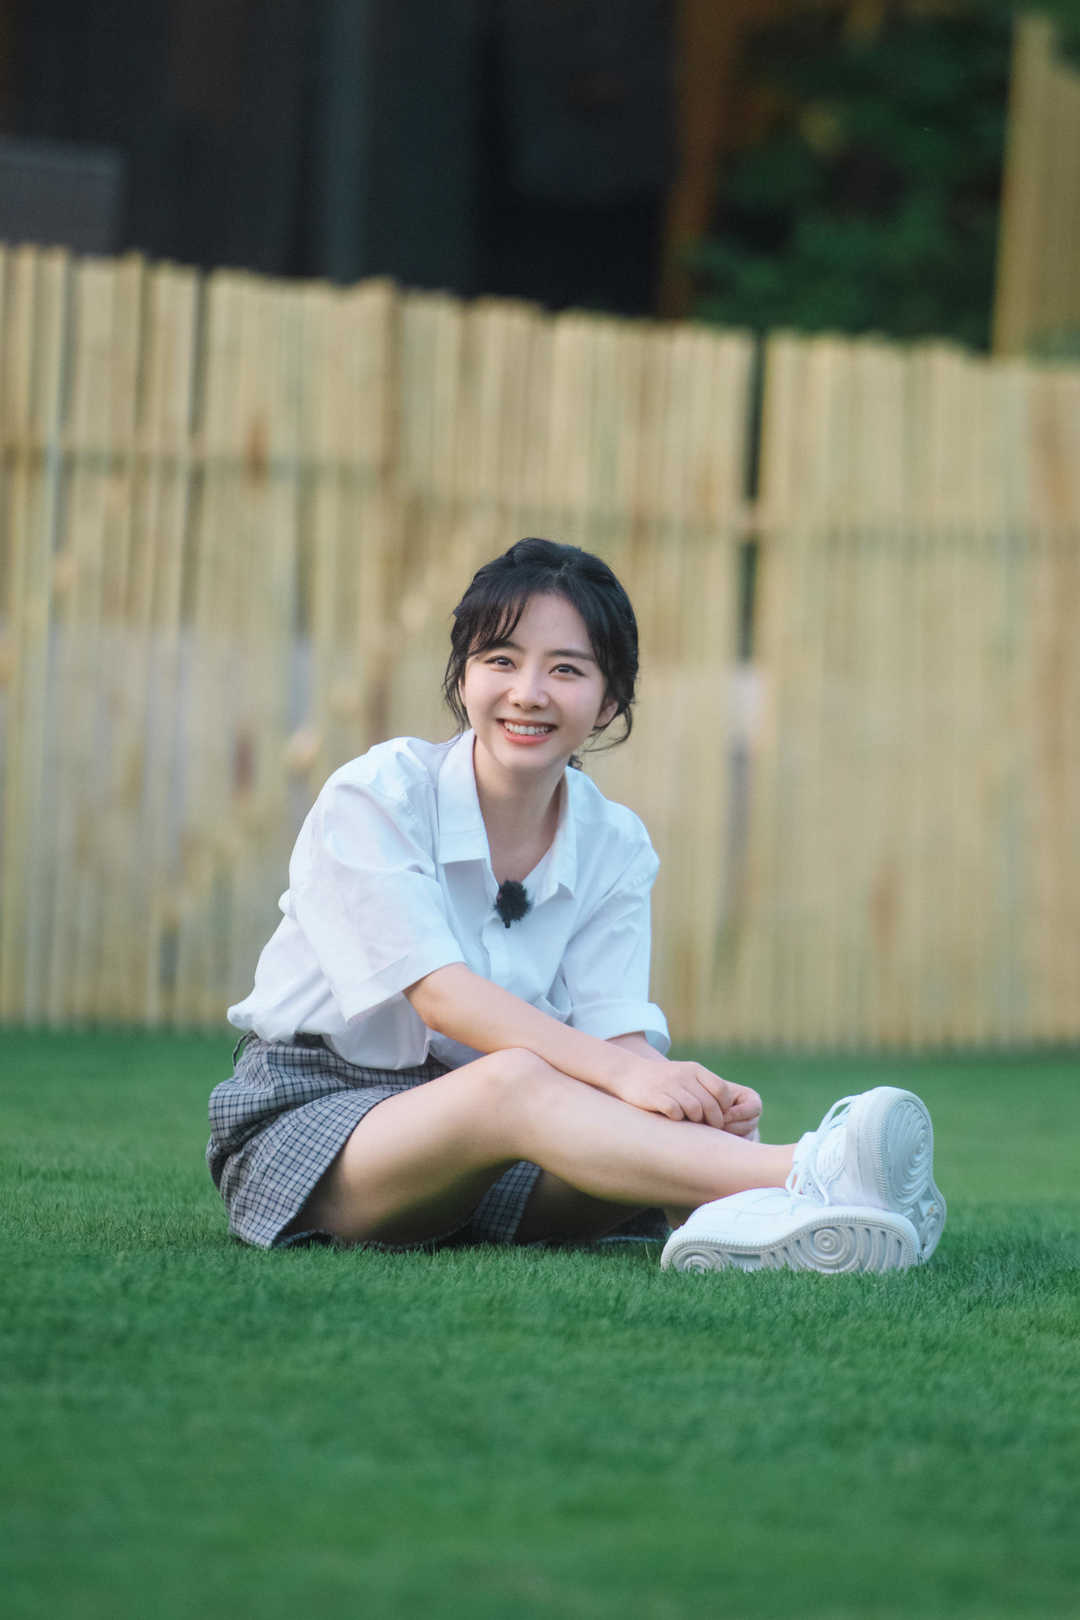
\includegraphics[width= .8\textwidth]{fiancee.jpg}
% 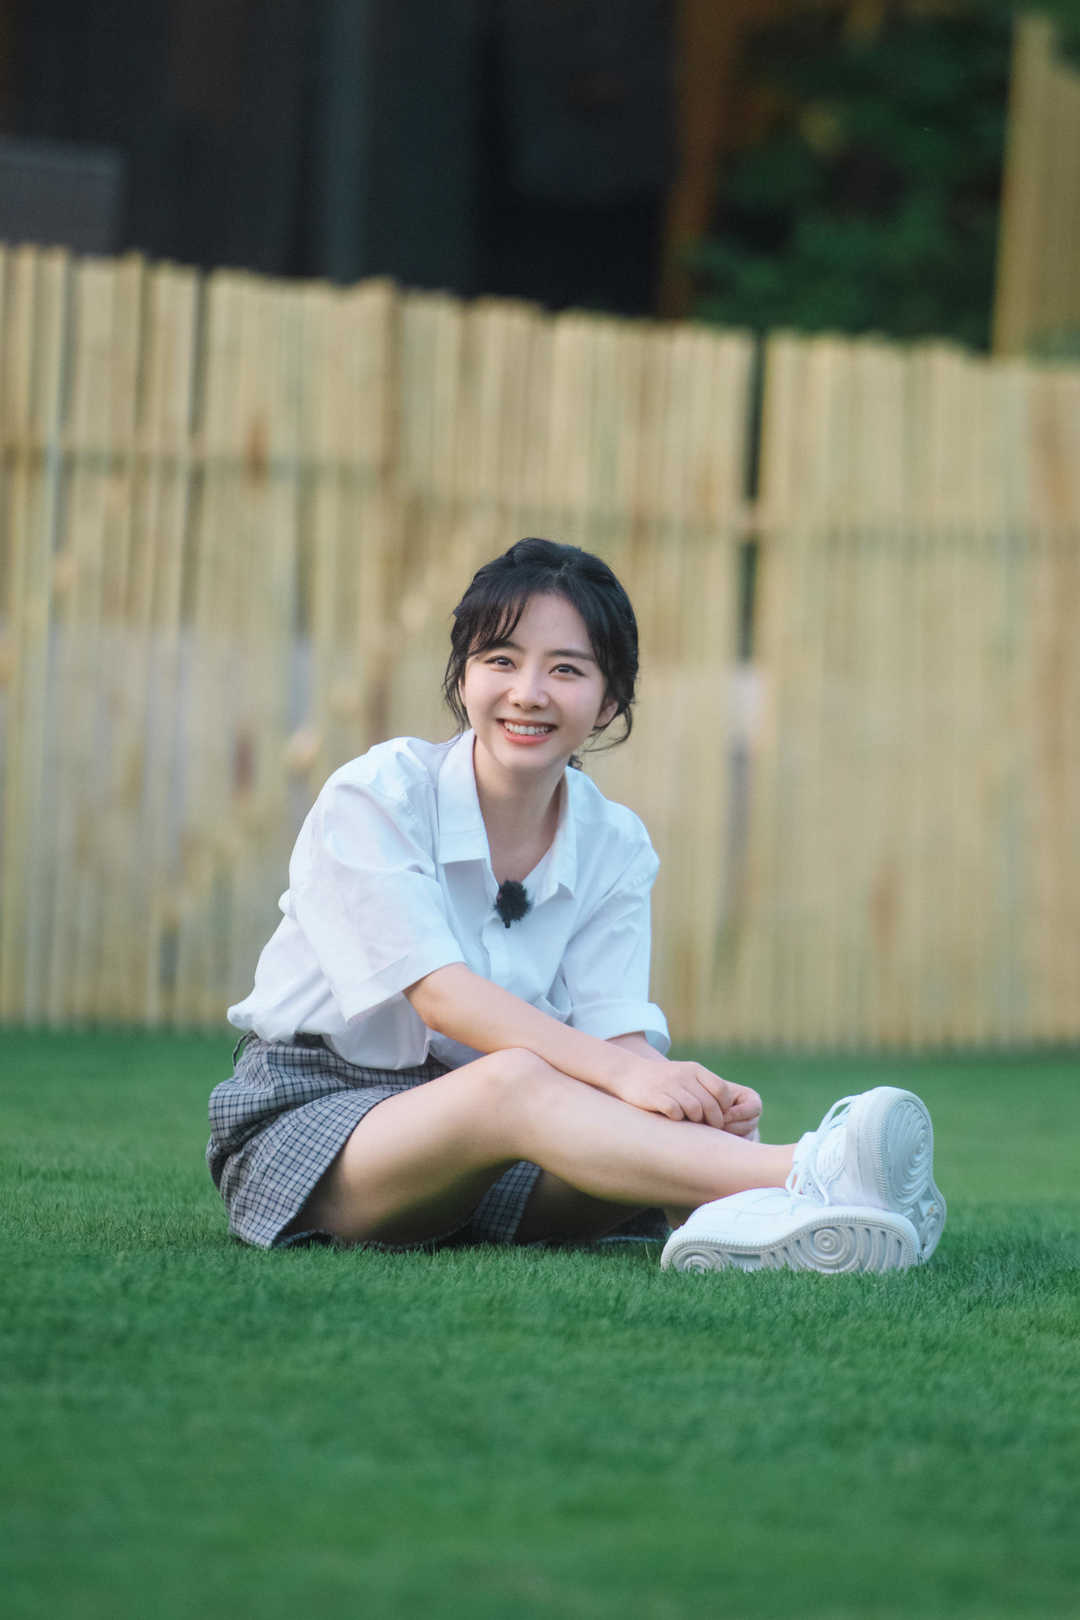
\includegraphics[width= 0.8\textwidth]{fiancee.jpg}


%%% Picture.tex
% \documentclass{article}
% \usepackage{xeCJK}
% \usepackage{graphicx}
% \setCJKmainfont{SimSun}
% \begin{document}
% 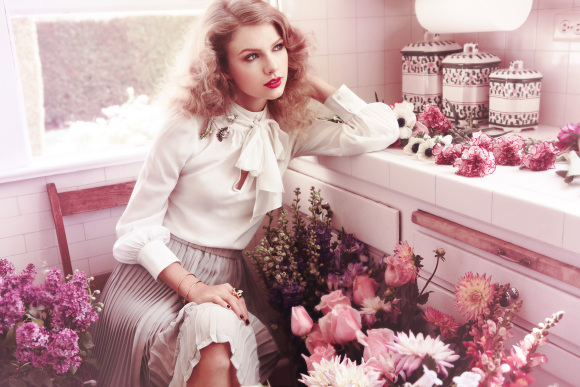
\includegraphics[width=.8\textwidth]{TaylorSwift-1.jpg}
% \end{document}

%%% Tabular.tex
% \documentclass{article}
% \usepackage{xeCJK}
% \setCJKmainfont{SimSun}
% \begin{document}
% \begin{tabular}{|l|cr|}
% \hline
% 操作系统& 发行版 & 编辑器\\
% \hline
% Windows & MikTeX & TexMakerX \\
% \hline
% Unix/Linux & teTeX & Kile \\
% \hline
% Mac OS & MacTeX & TeXShop \\
% \hline
% 通用& TeX Live & TeXworks \\
% \hline
% \end{tabular}
% \end{document}


%%% Tabular 2
% \documentclass{article}
% \usepackage{xeCJK}
% \setCJKmainfont{SimSun}
% \begin{document}
% \begin{tabular}{llr}
%     \multicolumn{2}{c}{Item} \\
%     Animal & Description & Price (\$)\\
%     Gnat & per gram & 13.65 \\
%          & each & 0.01 \\
%      Gnu & stuffed & 92.50 \\
%     Emu & stuffed & 33.33 \\
%     Armadillo & frozen & 8.99 \\
% \end{tabular}
% \end{document}


%%% float
% \documentclass{article}
% \usepackage{xeCJK}
% \usepackage{graphicx}
% \usepackage[colorlinks=false]{hyperref} % clickable links for jumping
% \setCJKmainfont{SimSun}
% \begin{document}
% \noindent
% I love You! \quad\quad I love You! \quad\quad I love You! \quad\quad I love You!\\
% I love You! \quad\quad I love You! \quad\quad I love You! \quad\quad I love You!
% % htbp 选项用来指定插图的理想位置
% % 这几个字母分别代表 [h]ere, [t]op, [b]ottom, float [p]age
% \begin{figure}[htbp]
% \centering
% % 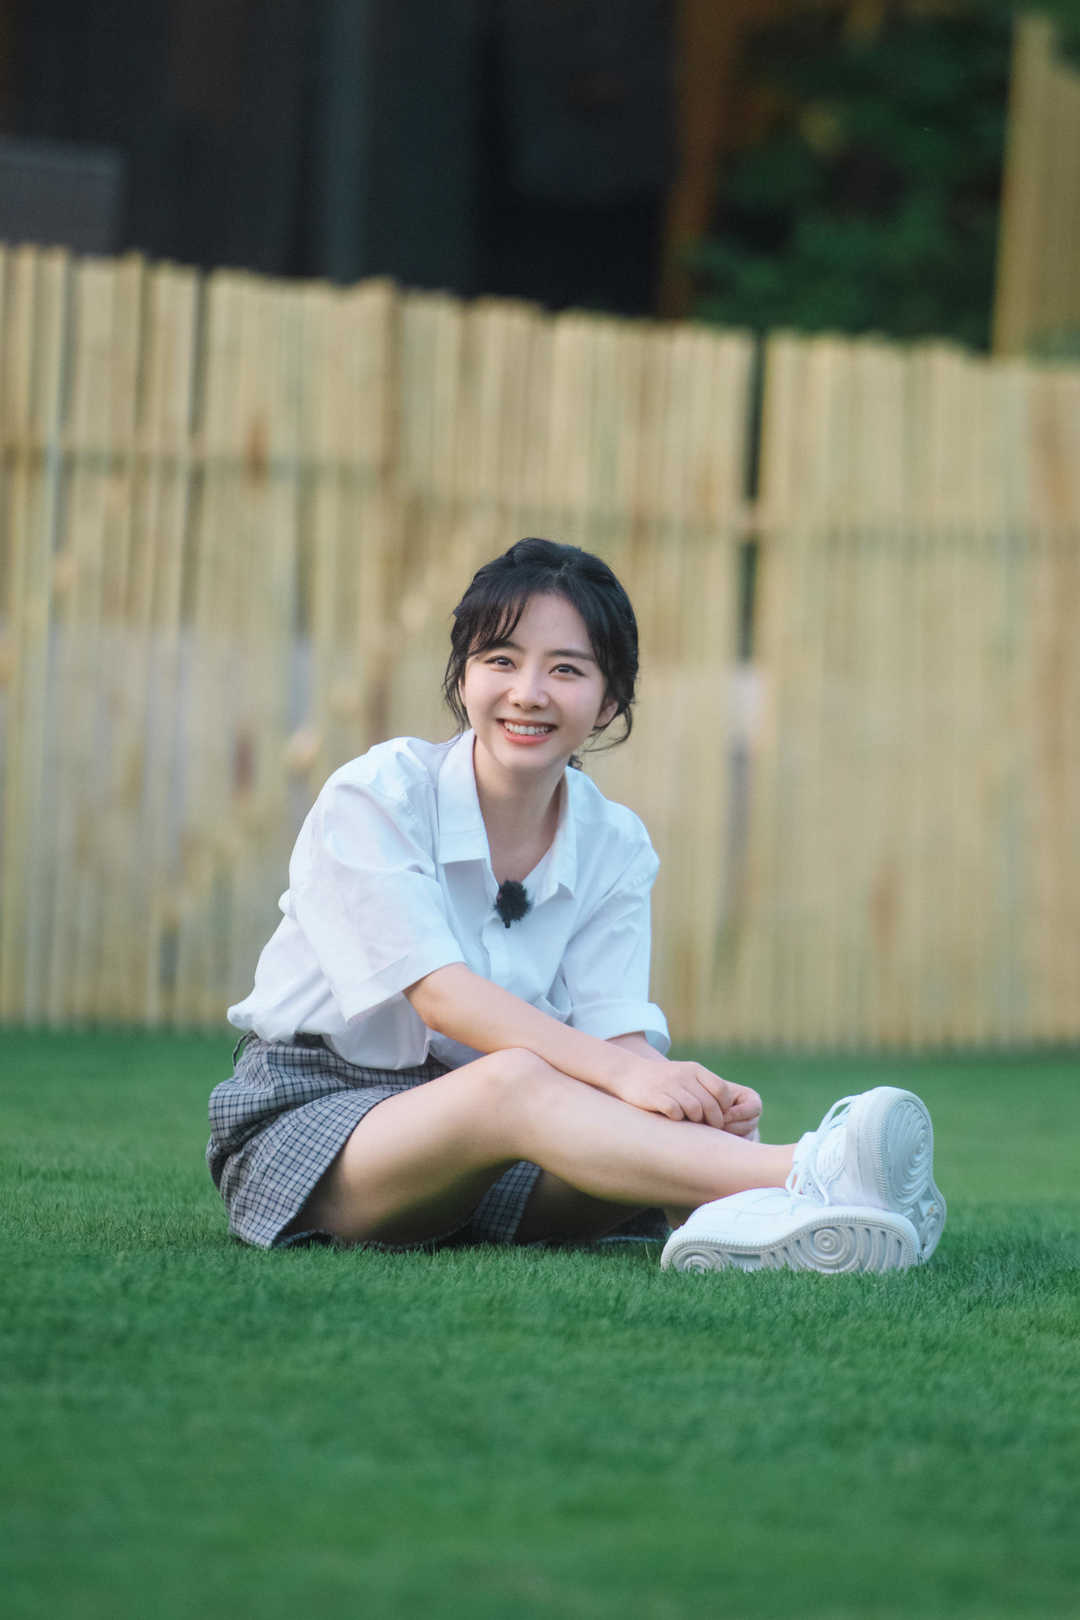
\includegraphics[width=8cm]{fiancee.jpg}
% 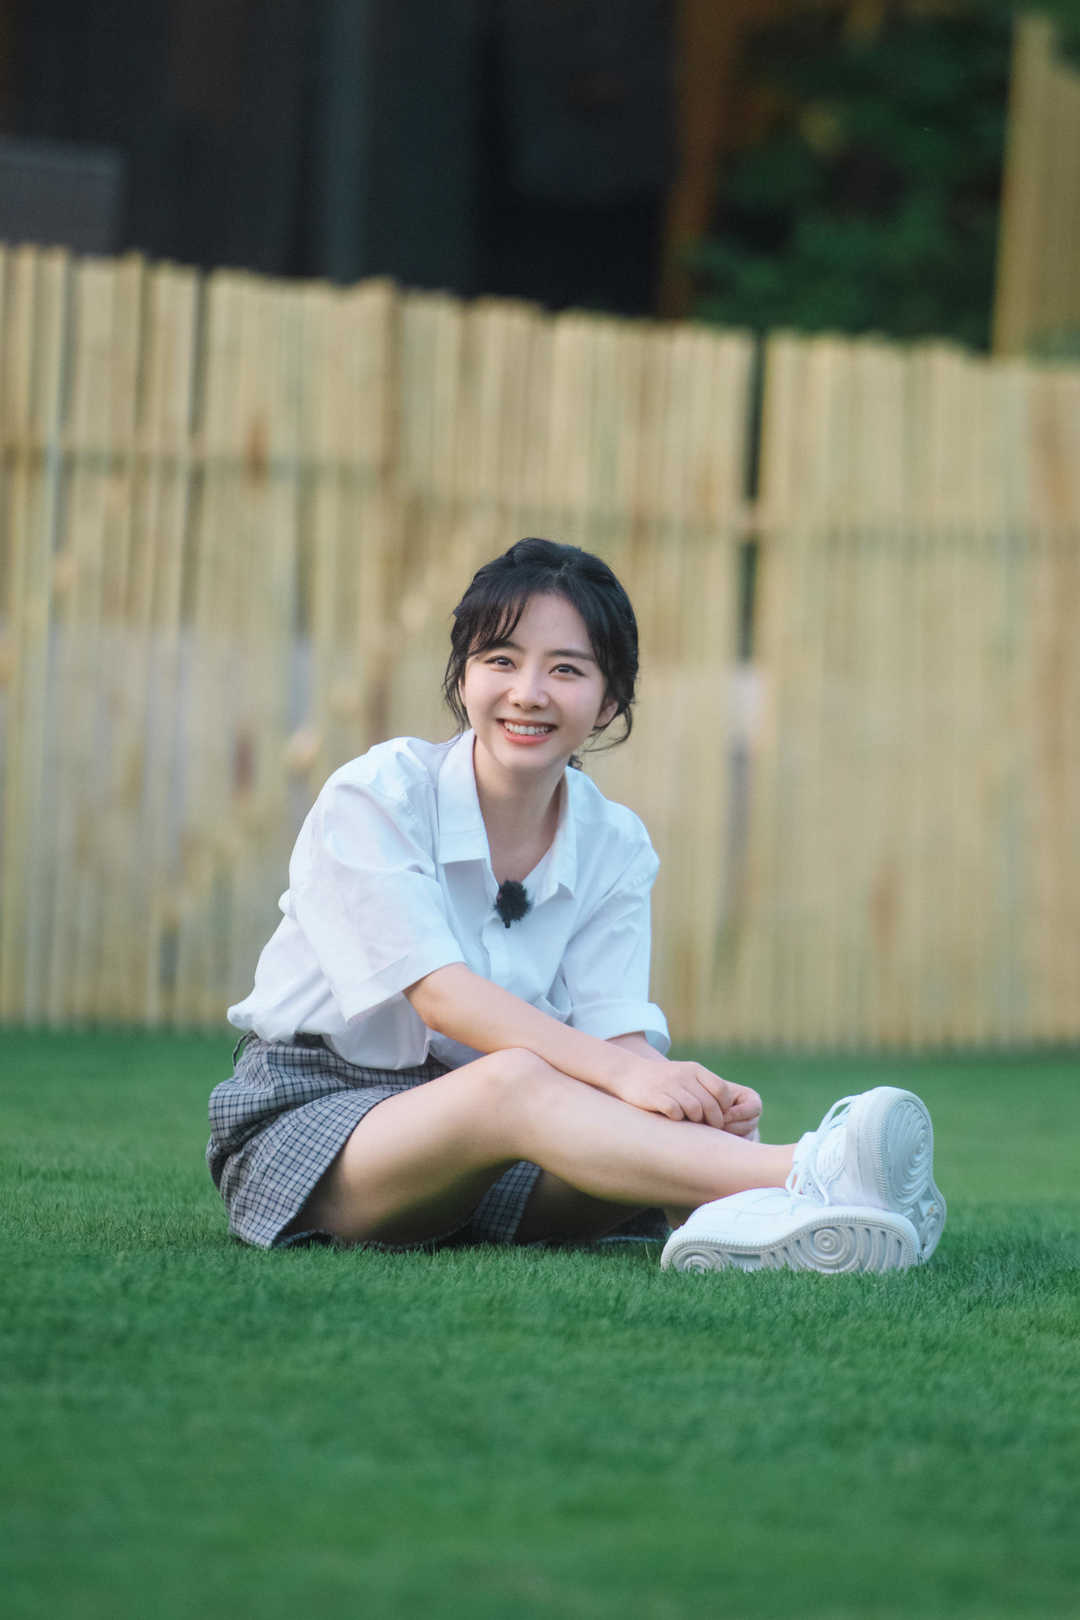
\includegraphics[width=4cm,height=10cm,keepaspectratio]{fiancee.jpg}
% % label{} 里面的内容随意,只要之后\ref{}引用的时候一模一样就可以
% \caption{有图有真相}\label{fig:fiancee}
% \end{figure}

% double click (figure~\ref{fig:fiancee}) to jump.
% \end{document}


%%% Page_Margins.tex
% \documentclass{article}
% \usepackage{xeCJK}
% \usepackage{geometry}
% \setCJKmainfont{SimSun}
% \geometry{papersize={20cm,15cm}}
% \geometry{left=1cm,right=2cm,top=2cm,bottom=4cm}
% \begin{document}
% 设置页边距,推荐使用 geometry 宏包。可以在这里查看它的说明文档。
% 设置页边距,推荐使用 geometry 宏包。可以在这里查看它的说明文档。
% 设置页边距,推荐使用 geometry 宏包。可以在这里查看它的说明文档。
% 设置页边距,推荐使用 geometry 宏包。可以在这里查看它的说明文档。
% \end{document}


%%% @{command} defines the space before and after one column
%%% !{command} defines what should be printed as vertical line
% \documentclass[border=14pt]{standalone}
% \usepackage{array}
% \begin{document}
% \begin{tabular}{@{dimen} c!{rule} c!{\vrule width 5pt}}
% \hline
% foo & bar\\
% \hline
% \end{tabular}
% \end{document}


%%% Headers_Footers.tex
% \documentclass{article}
% \usepackage{graphicx}
% \usepackage{fancyhdr}
% \pagestyle{fancy}
% \fancyhf{} % clear all header and footer fields
% \lhead{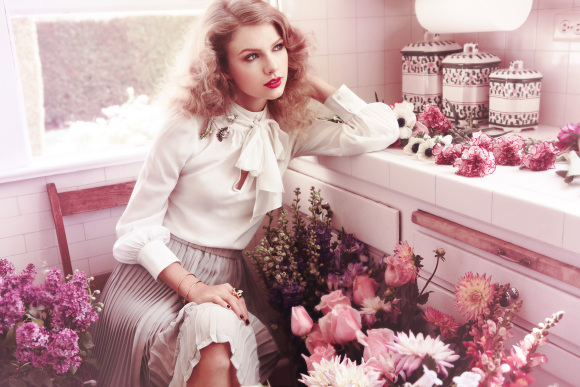
\includegraphics[height=2.5\baselineskip]{TaylorSwift-1.jpg}}
% \chead{\today}
% \rhead{\tiny \begin{tabular}[b]{@{}c@{}}Some College\\Some place\\Some department\\Some date\end{tabular}}
% \lfoot{}
% \cfoot{\thepage}
% \rfoot{}
% \renewcommand{\headrulewidth}{0.4pt}
% \renewcommand{\headwidth}{\textwidth}
% \renewcommand{\footrulewidth}{0pt}
% \begin{document}
% \noindent I love You!\\
% This's tragic story. Because I'm unrequited.
% \end{document}


%%% 杂项.tex
%% 设置成1.5倍行间距
% \usepackage{setspace}
% \onehalfspacing
%% 段间距,增加0.4em,负数就是减小了
% \addtolength{\parskip}{.4em}


%%% 各种字体.tex
%%% this file can be compiled with xelatex command
\documentclass[12pt, a4paper]{article}
\usepackage{fontspec}
\usepackage[slantfont, boldfont]{xeCJK}

\setmainfont{Microsoft YaHei}
\setsansfont{Comic Sans MS}
\setmonofont{Courier New}
\setCJKmainfont{Microsoft YaHei}
\setCJKmonofont{SimSun}
\setCJKsansfont{YouYuan}

% set up Chinese font, the font must be valid on your system
% correct line break for chinese
\XeTeXlinebreaklocale{zh}
\XeTeXlinebreakskip=0pt plus 1pt

\title{红楼梦}
\author{曹雪芹}
\date{\today}
\begin{document}
\maketitle
\begin{center}
满纸荒唐言\\
一把辛酸泪\\
都云作者痴\\
谁解其中味\\
\end{center}
\begin{verse}
\texttt{Stray birds of summer come to my window\\ to sing and fly away}. \\
\textsf{And yellow leaves of autumn, which have no songs}, \\
\textrm{flutter and fall there with a sign}.\\
\hfill \emph{RabindranathTagore}
\end{verse}
\begin{verse}
\texttt{夏天的飞鸟},\textsf{飞到我的窗前唱歌},\textrm{又飞去了}。\\
秋天的黄叶,它们没有什么可唱,只叹息一声,飞落在那里。\\
\hfill \emph{罗宾德拉纳特·泰戈尔}
\end{verse}
\end{document}

